In this appendix, I will explain in detail the process I undertook during the systematic review of literature (SRL) during my thesis project, highlighting the search queries I used, the outcomes of those queries, and the relative data sources. 

\section{Research Methodology}
\label{sec:resmetodologies}
In this thesis, a comprehensive literature review was utilized as a research methodology because it offers a structured and meticulous process for identifying, assessing, and examining existing resources to explore a specific research topic or question. The procedure used is the one illustrated in \citeauthor{budgen_performing_2006} (2006). In addition, I used also the snowballing approach defined in \citeauthor{wohlin_guidelines_2014} (2014).
\begin{figure}
\begin{center}
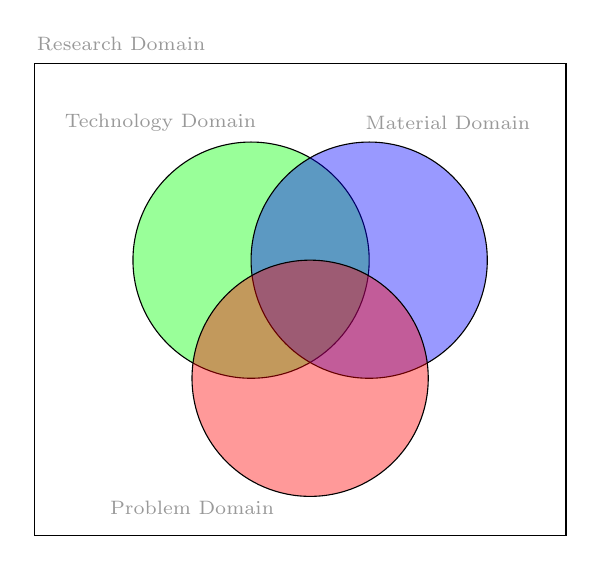
\begin{tikzpicture}[scale=0.5]
%% You can adjust the opacity here. For venn diagrams it is convenient to have a low opacity so that you can see intersections
	\begin{scope} [fill opacity = .4]
%% The draw command knows a lot of shapes. To make a rectangle you just need to specify two diagonal corners. Make sure you always have a semicolon at the end of your draw commands, otherwise latex flips out.
    \draw (-7,6) rectangle (6.5,-6);
%% Similarly, you can make a circle by specifying the center and then the radius. You can also add a fill color, but if you're printing in black and white you'll probably want to remove that line.
    \draw[fill=green, draw = black] (-1.5,1) circle (3);
    \draw[fill=blue, draw = black] (1.5,1) circle (3);
    \draw[fill=red, draw = black] (0,-2) circle (3);
%% We can use the node command to label points. If you put your cursor on "LARGE" or "textbf" a box will drop down with size and text style options.
    \node at (-4.8,6.5) {\scriptsize{Research Domain}};
    \node at (-3.8,4.5) {\scriptsize{Technology Domain}};
    \node at (3.5,4.5) {\scriptsize{Material Domain}};
    \node at (-3,-5.3) {\scriptsize{Problem Domain}};
    \end{scope}
\end{tikzpicture}
\end{center}
\caption{Research domain.} \label{fig:resdomains}
\end{figure}

\paragraph{Research terms.} To find the relevant search terms and phrases, I used the snowballing approach \cite{wohlin_guidelines_2014}. The schema of the aforementioned approach is described in Fig. \ref{fig:pallinacoca}. I found alternative spellings and/or synonyms for all major terms and phrases. Specifically, I identified three domains for terms usage: the technological domain, outlined by the PBF processes discussed throughout the thesis; the materials domain associated with the PBF processes; and the problem domain, focusing on the detection of hot spots. I used terms from the intersection of these three domains to structure the search queries for the databases mentioned subsequently. See Fig. \ref{fig:resdomains}.
\begin{itemize}
    \item \textbf{Technological domain:} powder bed fusion, L-PBF, PBF, electron beam melting, selective laser sintering, SLS, EBM.
    \item \textbf{Material domain:} metal, alloy, metal powder.
    \item \textbf{Problem domain:} hot spot, detection, machine learning, ML.
\end{itemize}

\paragraph{Research sources} In an SLR, selecting appropriate resources to search for material is critical. All available literature relevant to the scope of the thesis was selected and searched using the following resources:
\begin{itemize}
    \item Google Scholar (\href{https://scholar.google.com}{https://scholar.google.com})
    \item IEEE Xplore digital library (\href{https://ieeexplore.ieee.org}{https://ieeexplore.ieee.org})
    \item Scopus (\href{https://www.scopus.com/}{https://www.scopus.com/})
\end{itemize}

\paragraph{Performed queries.} In this paragraph, I will report all the queries used on the different sources for the research. \\[1.5ex]
Query performed on Scopus:
\begin{tcolorbox}
\footnotesize
((Powder AND bed AND fusion) OR PBF OR L-PBF OR (electron AND beam AND melting) OR (selective AND laser AND sintering) OR SLS OR EBM) AND (metal OR alloy OR (metal AND powder)) AND  (hot AND spot*) AND (ML OR (machine AND learning)) AND ((defect* OR anomal*) AND detection) AND ((additive AND manufacturing) OR AM)
\end{tcolorbox}
Since IEEE Xplore digital does not have the structured query Scopus does, I decided to perform multiple queries. Query performed on IEEE Xplore digital library:
\begin{tcolorbox}
\footnotesize
"All Metadata":"powder bed fusion" AND "metal" AND "hot spot*" AND "detection"
\end{tcolorbox}
\begin{tcolorbox}
\footnotesize
"All Metadata":"electron beam melting" AND "metal" AND "hot spot*" AND "detection"
\end{tcolorbox}
\begin{tcolorbox}
\footnotesize
"All Metadata":"selective laser sintering" AND "metal" AND "hot spot*" AND "detection"
\end{tcolorbox}
Dued to query search system of Google Scholar, I used same queries.



\section{Research result and selection process.}
\label{sec:resresults}
\begin{figure}
    \centering
    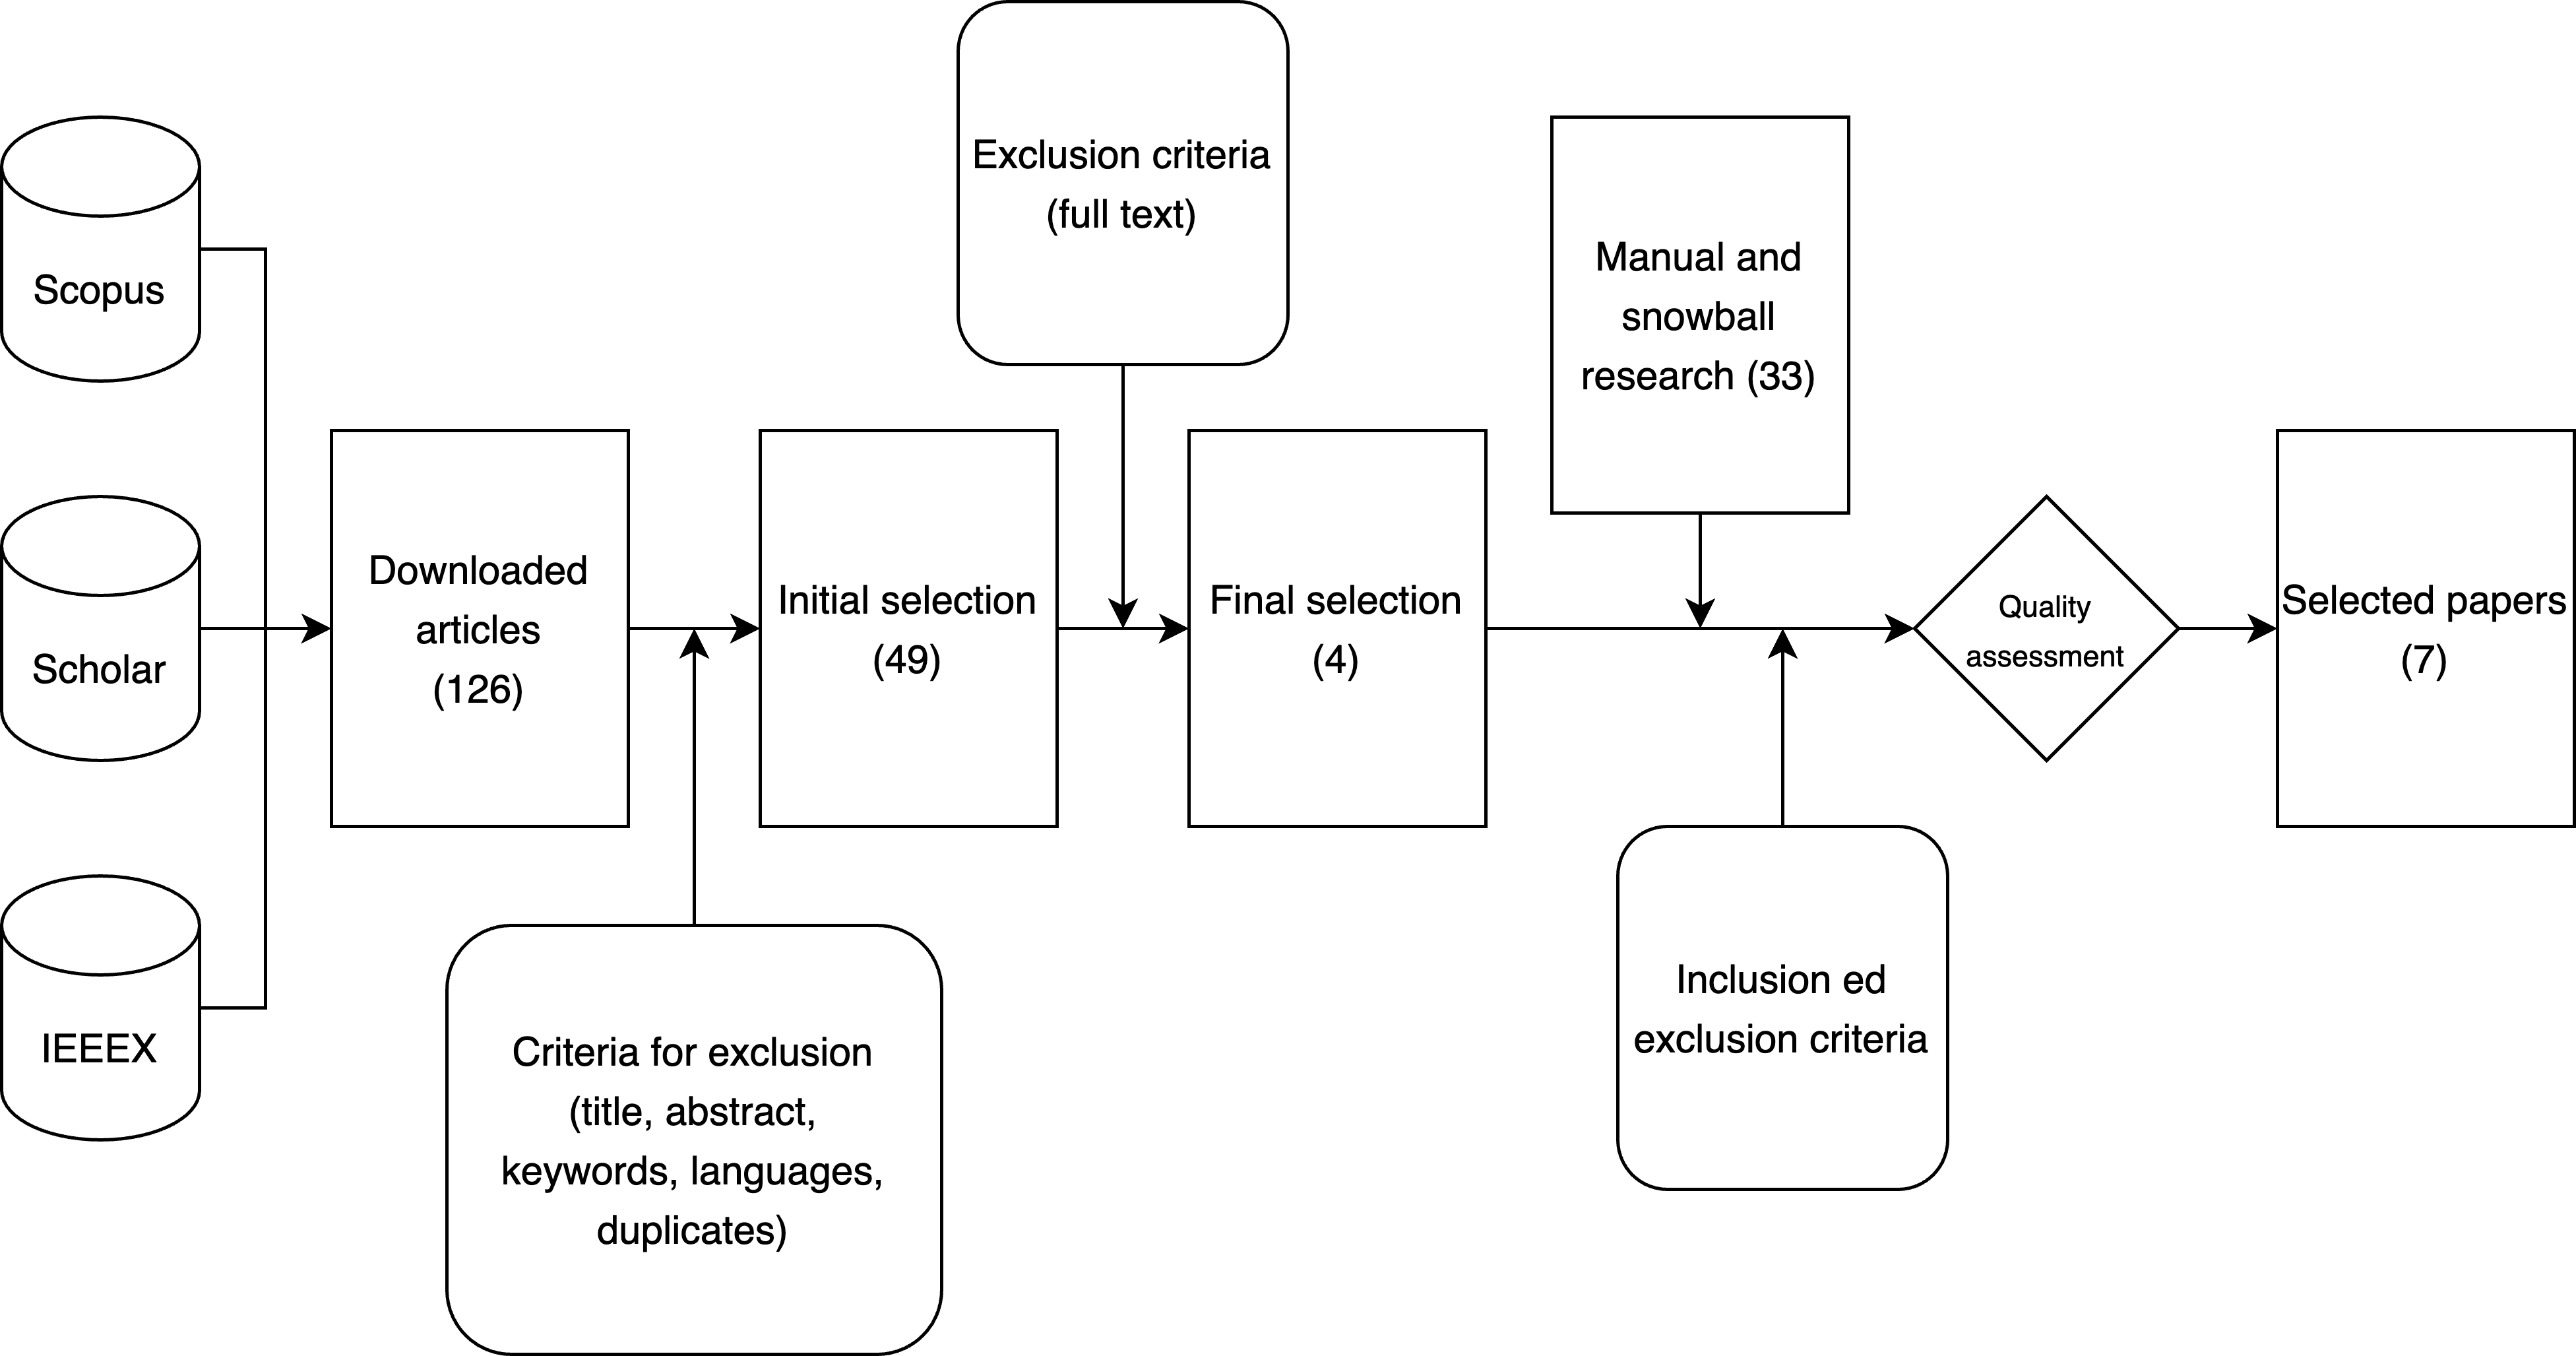
\includegraphics[scale=0.2]{Images/selezioncina.png}
    \caption[Papers selection procedure.] {Papers selection procedure.}
    \label{fig:selezioncina}
\end{figure}
During the SLR, I used some exclusion criteria and inclusion criteria to select the final papers for the research. 
An article has to meet the following criteria to be useful in answering our research questions.
\paragraph{Exclusion criteria.} These are the exclusion criteria I decided to use:
\begin{itemize}
    \item Papers about anomalies detection methods other than machine learning or deep learning;
    \item Papers that aren’t available in their whole;
    \item Papers written in a language besides English;
    \item Papers in a state besides "Final Release".
\end{itemize}
\paragraph{Inclusion criteria.} On the other hand, I included the following:
\begin{itemize}
    \item All the articles, written in English, report machine learning or deep learning technique for  hot spots detection;
    \item All papers, journal, conference, workshop, and short papers but books.
    \item All articles about the review of possible defects in PBF.
\end{itemize}
For the last point, these are the papers I used to write \emph{Chapter ~\ref{ch:defects}} and to perform the snowballing procedure explained before.

\begin{figure}
    \centering
    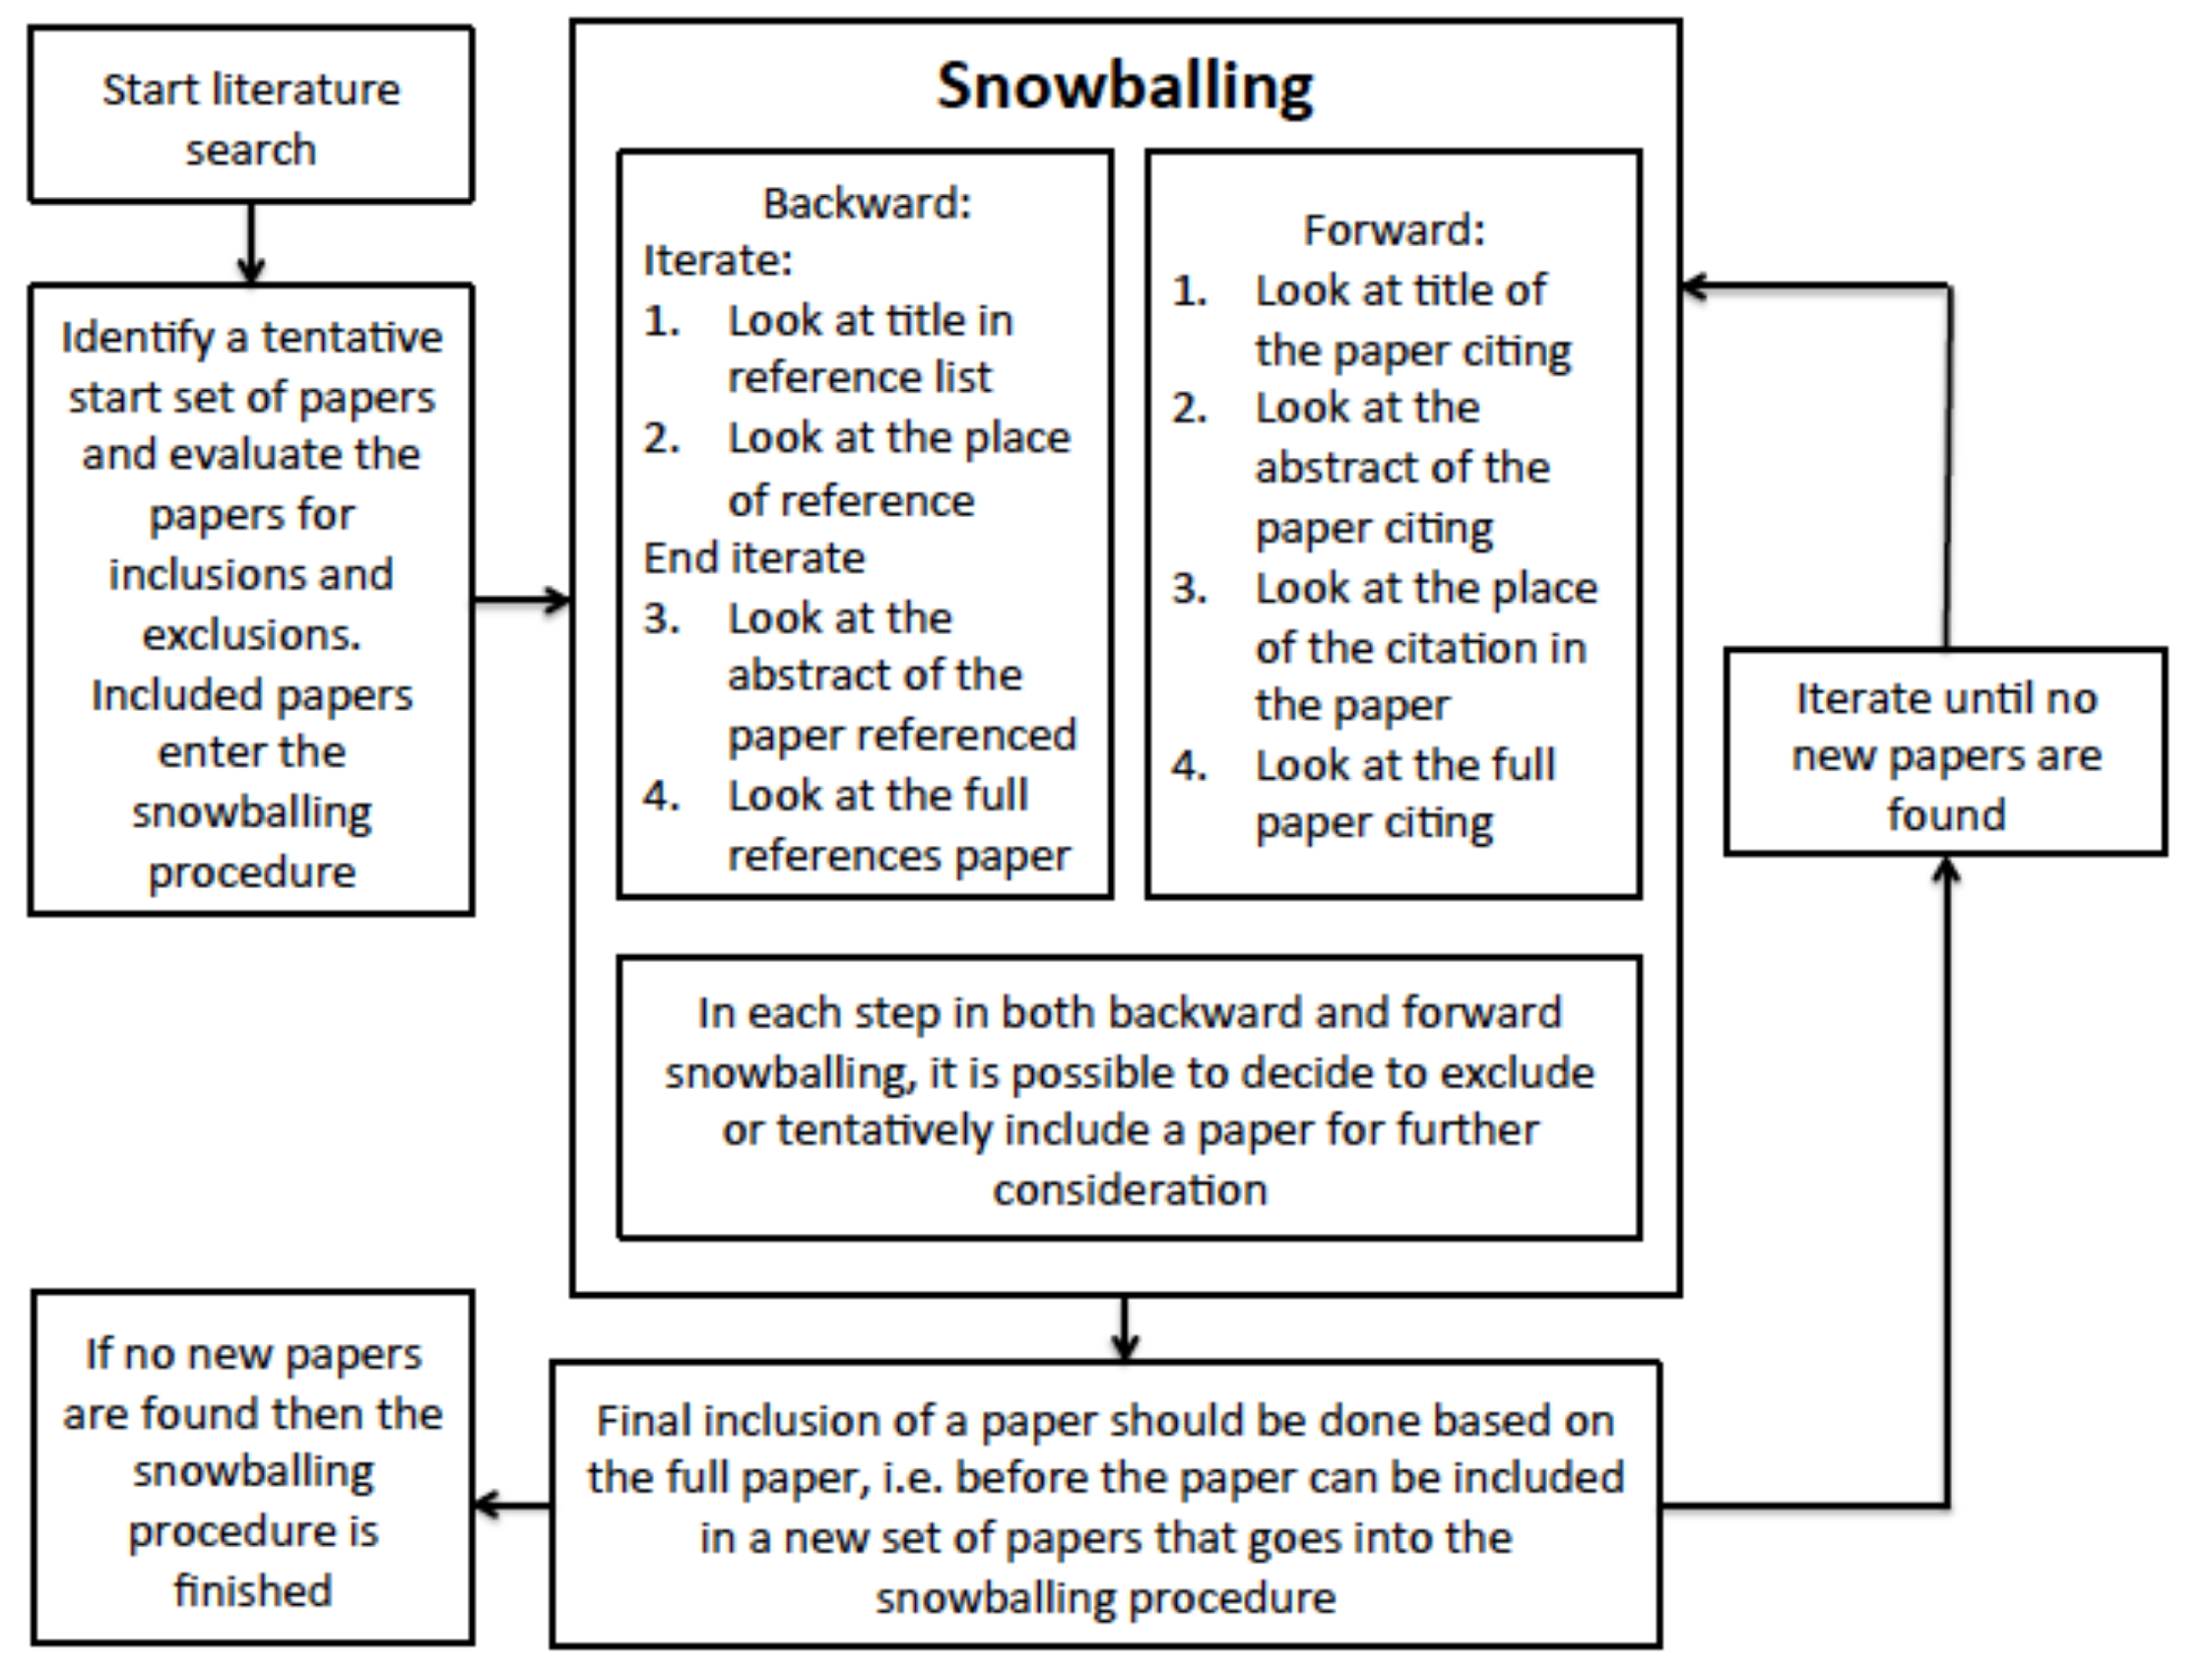
\includegraphics[scale=0.25]{Images/pallinadicoca.png}
    \caption[Snowballing procedure.] {The schema of the snowballing procedure \cite{wohlin_guidelines_2014}.}
    \label{fig:pallinacoca}
\end{figure}
